\documentclass[tikz,border=4pt]{standalone}
\usepackage{amsmath,amssymb}
\usetikzlibrary{arrows.meta}

\begin{document}
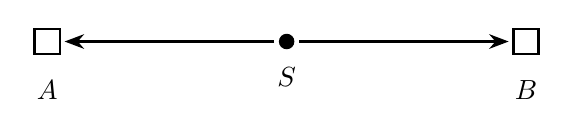
\begin{tikzpicture}[
  >=Stealth,
  font=\normalsize,
  axis/.style={line width=0.4pt},
  curve/.style={line width=0.9pt}
]
  % Source at center
  \fill (0,0) circle (2.8pt);
  \node[below=6pt] at (0,0) {$S$};

  % Detector A (left) and B (right)
  \draw[curve] (-3.2,-0.16) rectangle (-2.88,0.16);
  \node[below=6pt] at (-3.04,-0.16) {$A$};

  \draw[curve] (2.88,-0.16) rectangle (3.2,0.16);
  \node[below=6pt] at (3.04,-0.16) {$B$};

  % Arrows from source to detectors
  \draw[curve,->] (-0.16,0) -- (-2.82,0);
  \draw[curve,->] (0.16,0) -- (2.82,0);
\end{tikzpicture}
\end{document}
